\documentclass[journal, a4paper]{IEEEtran}
\usepackage{cite}
\usepackage{amsmath,amssymb,amsfonts}
\usepackage{graphicx}
\usepackage{textcomp}
\usepackage{xcolor}
\usepackage{float}

\begin{document}

\title{Explaining the Black Box: A Study on the Application of Explainable Artificial Intelligence (XAI) Techniques to Machine Learning Models}
\author{
    \large
    \IEEEauthorblockN{Magdalena~Pakuła\IEEEauthorrefmark{1}}
    and
    \IEEEauthorblockN{Jakub~Pawlak\IEEEauthorrefmark{2}}\\[1ex]
    \normalsize
    \IEEEauthorblockA{
        WFTIMS, Politechnika Łódzka\\
        Email: \IEEEauthorrefmark{1}254220@edu.p.lodz.pl, \IEEEauthorrefmark{2}254222@edu.p.lodz.pl
    }
}


\maketitle

\begin{abstract}
    The increasing reliance on artificial neural networks in various applications has raised concerns about their \textit{black box} nature, making it challenging to understand the decision-making processes behind their predictions.
    This report addresses this challenge by exploring the application of so-called Explainable Artificial Intelligence (XAI) techniques to machine learning models.
    Specifically, we employ local explanation approaches, including attributions and counterfactual examples, using the Captum library in the PyTorch such as LIME, saliency maps or integrated gradients techniques.
    Our study aims to shed light on the selected trained models, providing a deeper understanding of how they make predictions and present those findings in this report
\end{abstract}

\section{Introduction}\label{sec:introduction}

\IEEEPARstart{A}{rtificial} neural networks (ANNs) have revolutionized various industries and applications, from healthcare to finance, by enabling accurate predictions and decision-making.
However, the increasing reliance on these models has also raised concerns about their \textit{black box} nature, making it challenging to understand the decision-making processes behind their predictions.
This opacity can lead to a lack of trust in the models, as well as difficulties in identifying biases and errors.
To address this challenge, Explainable Artificial Intelligence (XAI) techniques have emerged as a crucial step towards building more transparent and accountable machine learning models.
By applying XAI methods, we can gain insights into the internal workings of complex models, providing a deeper understanding of how they make predictions and enabling more informed decision-making.
This project aims to explore the application of XAI techniques to machine learning models, specifically focusing on local explanation approaches such as attributions and counterfactual examples.
By shedding light on the previously trained models, we aim to provide a better understanding of how they make predictions and contribute to the development of more transparent and trustworthy AI systems.

\section{Related Work}\label{sec:related-work}
This study explores various techniques used to enhance the interpretability and transparency of Artificial Neural Networks (ANNs) through Explainable Artificial Intelligence (XAI) methods.

The first paper in this domain that we examined was~\cite{ribeiro2016should} by Ribeiro et al.
This paper was the first to publicly introduce the Local Interpretable Model-Agnostic Explanations (LIME) framework, which generates local, interpretable explanations for the predictions of any machine learning model.
The key idea behind LIME is to approximate the original complex model with an interpretable model that is locally faithful to the prediction of interest.
This paper was an important step in the development of XAI techniques, as it demonstrated the feasibility and utility of interpretable explanations.

Since then, the field of XAI has continued to evolve, with many other techniques (e.g. SHAP, TCAV, GradCAM) being proposed to enhance the transparency and interpretability of AI systems.
However, LIME provides local explanations that are specific to individual predictions and while useful, these local explanations may not offer a comprehensive understanding of the model's overall behavior~\cite{NIPS2017_8a20a862}.

Different approach for understanding model predictions include saliency maps, thoroughly explained by Simonyan et al.~\cite{Simonyan14a}.
This paper presents the method, which computes the gradient of the score of the predicted class with respect to the input image.
The gradient essentially measures how small changes in each pixel value of the image will affect the output score.
The absolute values of these gradients are taken to represent the importance of each pixel and pixels with larger gradient magnitudes are considered more important for the classification decision.
Therefore, saliency maps effectively highlight discriminative image regions and objects, which are easily interpretable by a human eye.

To provide a broader view and better understanding, we reviewed another influential paper by Sundararajan et al.~\cite{ribeiro2016should}, which provided an alternative surrogate-based methods like LIME or sometimes misleading saliency maps~\cite{adebayo2018sanity}.
The authors introduce and demonstrate the usefulness of integrated gradients through various case studies, including image classification.
They show that this method can provide meaningful and intuitive explanations of the model's predictions, which can be valuable for tasks like feature importance analysis.
Additionally, the authors compare integrated gradients method to other gradient-based attribution methods, such as saliency maps and deconvolution, and highlight the advantages of it in terms of desirable properties for explanations.

Furthermore, counterfactuals are an essential aspect of XAI, as they provide a way to evaluate the robustness of a model's predictions by considering what would have happened if certain conditions had been different~\cite{adebayo2018sanity}.
This is particularly important in high-stakes applications, such as healthcare or finance, where the consequences of incorrect predictions can be severe.
For example, Adebayo et al.~\cite{adebayo2018sanity} evaluated the reliability of saliency maps on the MNIST and CIFAR-10 image classification datasets by applying counterfactual perturbations like rotation and occlusion to the input images.
They found that many popular saliency map methods failed to provide faithful explanations, underscoring the importance of using counterfactuals to assess the robustness of model predictions.

Those papers provide a solid ground for experimenting on different models with different methods in order to fully understand models predictions.
\section{Methodology}\label{sec:methodology}

\subsection{ANN models}\label{subsec:ann-models}

This experiment will be conducted on various types of data and ANN models for testing the versatility of different XAI methods.
Models used in this experiment:
\begin{itemize}
    \item \textbf{MLP models:}
          \begin{itemize}
              \item \textbf{Iris flowers, wines, and breast cancer:}
                    \begin{itemize}
                        \item Two hidden layers with 64 and 32 neurons respectively
                        \item ReLU activation function
                        \item Adam optimizer
                    \end{itemize}

              \item \textbf{Handwritten numbers from the MNIST dataset:}
                    \begin{itemize}
                        \item Two linear layers for mapping input features to hidden dimensions and output classes.
                        \item ReLU activation function
                    \end{itemize}
          \end{itemize}
    \item \textbf{CNN models:}
          \begin{itemize}
              \item \textbf{Handwritten numbers from the MNIST dataset:}
                    \begin{itemize}
                        \item Two convolutional layers with max pooling, Sigmoid activation and flatten operation for feature extraction
                        \item Three linear layers with Sigmoid activation for the classifier
                    \end{itemize}

              \item \textbf{Images from the CIFAR10 dataset:}
                    \begin{itemize}
                        \item Eight convolutional layers with batch normalization, max pooling, and ReLU activation for feature extraction
                        \item Three linear layers with ReLU activation for the classifier
                    \end{itemize}
          \end{itemize}

\end{itemize}

Additionally, for the MLP models recognizing handwritten numbers from the MNIST dataset were added three different feature extraction methods for each model:
\begin{itemize}
    \item \textbf{Flatten}: Converts the entire image into a single vector with 784 elements.
    \item \textbf{HOG} (Histogram of Oriented Gradients): Extracts features based on gradient orientations in local regions.
    \item \textbf{LBP} (Local Binary Patterns): Extracts features based on local texture patterns.
\end{itemize}

\subsection{Methods}\label{subsec:methods}
After a comprehensive review of the literature, our study focuses on exploring the critical factors influencing decision-making for specific inputs through the identification of attributions and counterfactuals using the following methods:

\begin{itemize}
    \item \textbf{LIME:} LIME is a model-agnostic technique that explains the predictions of any classifier by learning an interpretable model locally around the prediction.
          It approximates the decision boundary around a given input \( \mathbf{x} \) using a linear regression model:
          \[
              f(\mathbf{x}') = \boldsymbol{\theta} \cdot \mathbf{x}' + b
          \]
          where \( \boldsymbol{\theta} \) are the coefficients of the linear model and \( b \) is the bias term.
          By analyzing \( \boldsymbol{\theta} \), LIME identifies the important features that influenced the prediction \( f(\mathbf{x}') \).

    \item \textbf{Saliency Maps:}
          Saliency Maps highlight input features that are most influential for a model's prediction.
          They are computed by taking the absolute gradients of the output \( f(\mathbf{x}) \) with respect to the input \( \mathbf{x} \):
          \[
              S(\mathbf{x}) = \left|\frac{\partial f(\mathbf{x})}{\partial \mathbf{x}}\right|
          \]
          These maps provide insights into how sensitive the model's output is to changes in each input feature \( \mathbf{x}_i \).

    \item \textbf{Integrated Gradients:}
          Integrated Gradients attribute an output prediction to input features by integrating the gradients of the output \( f(\mathbf{x}) \) with respect to the input \( \mathbf{x} \) along a linear path from a baseline input \( \mathbf{x}' \) to the actual input \( \mathbf{x} \):
          \[
              \phi_i(\mathbf{x}) = (x_i - x'_i) \cdot \int_{\alpha=0}^{1} \frac{\partial f(\mathbf{x}' + \alpha (\mathbf{x} - \mathbf{x}'))}{\partial \mathbf{x}_i} \, d\alpha
          \]
          This method provides a comprehensive attribution of the model's prediction to each feature \( \mathbf{x}_i \), reflecting how each feature contributed to the final prediction.

    \item \textbf{Minimal Parameter Perturbation:}
          Minimal Parameter Perturbation is a technique that detects the smallest possible changes to the model parameters that can significantly change the model's output prediction.
          By identifying these minimal perturbations, we can gain valuable insights into the model's decision-making process and the features that are most critical for its predictions.
\end{itemize}

In addition, we employ SLIC (Simple Linear Iterative Clustering), a superpixel segmentation algorithm designed to partition images into compact, nearly uniform superpixels \( \{ S_k \} \).
SLIC achieves this through iterative clustering of pixels based on color similarity and spatial proximity, resulting in segments that enhance the interpretability of explainable AI (XAI) methods:
\[
    S(\mathbf{x}) = \arg \min_{S_k} \left( \|\mathbf{x} - \mathbf{m}_k\|^2 + \frac{\beta}{N_k} \sum_{\mathbf{x}' \in S_k} \|\mathbf{x} - \mathbf{x}'\|^2 \right)
\]
Here, \( \mathbf{m}_k \) denotes the mean color of superpixel \( S_k \), \( N_k \) represents the number of pixels in \( S_k \), and \( \beta \) serves to balance the importance between color and spatial proximities.

Upon presenting the results of this experiment, our aim is to uncover the underlying principles governing the models, with the goal of comprehending their overall behavior and underlying assumptions.

\section{Results}\label{sec:results}
This section presents the detailed findings and interpretations resulting from the application of various (XAI) methods to the chosen (ANN) models.
The analysis explores the factors influencing model predictions and enhances the interpretability of the results.

\subsection{MLP Models for Iris Flowers, Wines, and Breast Cancer}\label{subsec:experiment-other-datasets}
In this experiment the Local Interpretable Model-agnostic Explanations (LIME) method was employed to interpret the MLP models trained on the Iris, Wine and Breast Cancer dataset.
The results for the Iris dataset is as follows:
\begin{itemize}
    \item Example for class \textit{setosa} is predicted to be \textit{setosa} \\
          {\tiny
          \begin{verbatim}
     (sepal length (cm) <= -0.90, -0.298)
     (sepal width (cm) > 0.56, -0.202)
     (petal width (cm) <= -1.18, -0.074)
     (petal length (cm) <= -1.23, -0.074)
    \end{verbatim}
          }

    \item Example for class \textit{versicolor} is predicted to be \textit{versicolor} \\
          {\tiny
          \begin{verbatim}
     (sepal length (cm) > 0.67, 0.265)
     (0.13 < petal width (cm) <= 0.79, 0.074)
     (0.34 < petal length (cm) <= 0.76, 0.048)
     (-0.13 < sepal width (cm) <= 0.56, 0.001)
    \end{verbatim}
          }

    \item Example for class \textit{virginica} is predicted to be \textit{virginica} \\
          {\tiny
          \begin{verbatim}
     (petal width (cm) > 0.79, -0.219)
     (petal length (cm) > 0.76, -0.153)
     (-0.05 < sepal length (cm) <= 0.67, 0.104)
     (-0.13 < sepal width (cm) <= 0.56, -0.003)
    \end{verbatim}
          }
\end{itemize}

The interpretation of these findings suggests that the model predicts the class \textit{setosa} under specific conditions: when the sepal length is less than or equal to -0.90, the sepal width is greater than 0.56, the petal width is less than or equal to -1.18, and the petal length is less than or equal to -1.23.
In the datasets for Wine and Breast Cancer, exemplary results for different classes are as follows:

\begin{itemize}
    \item Example for class \textit{class 0} is predicted to be \textit{class 0} \\
          {\tiny
          \begin{verbatim}
     (alcohol > 0.84, -0.3134332679978472)
     (proline > 0.76, -0.264433236765466)
     (alcalinity_of_ash <= -0.69, -0.2251982383093865)
     (magnesium > 0.51', -0.11390769081064545)
     (proanthocyanins > 0.63, 0.08002171008559669)
     (-0.74 < nonflavanoid_phenols <= -0.18, -0.0482748726325857)
     (-0.66 < malic_acid <= -0.42, 0.047185845557030495)
     (-0.02 < ash <= 0.70, -0.04026117740681837)
     (od280/od315_of_diluted_wines > 0.79, -0.028340722297950868)
     (0.03 < hue <= 0.71, 0.02827508670536462)
    \end{verbatim}
          }
\end{itemize}

\begin{itemize}
    \item Example for class \textit{benign} is predicted to be \textit{benign} \\
          {\tiny
          \begin{verbatim}
     (worst texture <= -0.75, 0.21842857185438763)
     (-0.49 < area error <= -0.35, 0.11693408539760825)
     (texture error <= -0.69, -0.09013183858850903)
     (-0.62 < radius error <= -0.29, 0.08454431147818825)
     (mean texture <= -0.73, 0.07439644700747527)
     (-0.68 < worst compactness <= -0.27, -0.07233220030349469)
     (mean fractal dimension <= -0.72, -0.06777535676504395)
     (-0.59 < fractal dimension error <= -0.23, -0.06004003787372975)
     (-0.69 < compactness error <= -0.28, -0.049467416103845994)
     (-0.69 < worst fractal dimension <= -0.22, 0.04814347795800571)
    \end{verbatim}
          }
\end{itemize}

The values for all other classes follow a similar pattern as presented above.
These results demonstrate that the models base their predictions on key features such as sepal length, alcohol content, and worst texture etc.
The prominence of these features underscores their critical role in prediction, suggesting their significance as primary factors influencing model decisions.
Furthermore, these findings illustrate the models' capability to effectively distinguish between different classes based on these feature values.
Moreover, these insights are instrumental in identifying potential biases and inaccuracies within the model, thereby facilitating improvements in its performance.
For instance, by pinpointing features that contribute to bias towards certain classes, adjustments can be made to mitigate these biases and enhance the model's reliability and fairness.

\subsection{MNIST MLP classifier}\label{subsec:experiment-mnist-mlp}

\subsubsection{Flatten}

\begin{figure}[ht]\centering
    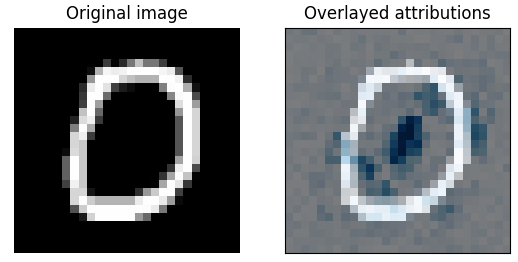
\includegraphics[width=.6\linewidth]{img/saliency_flat/0.png}
    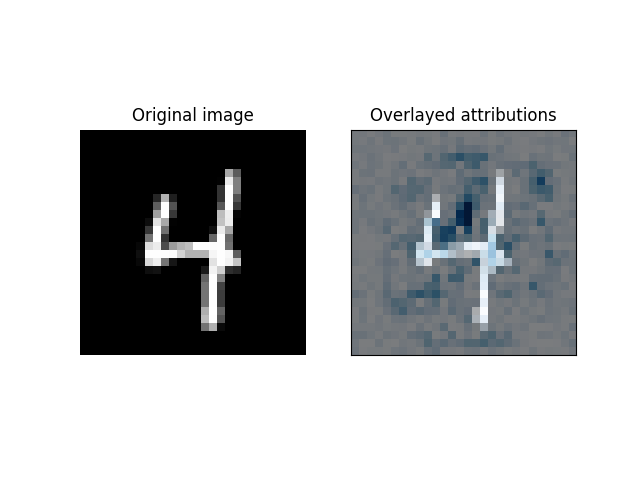
\includegraphics[width=.6\linewidth]{img/saliency_flat/4.png}
    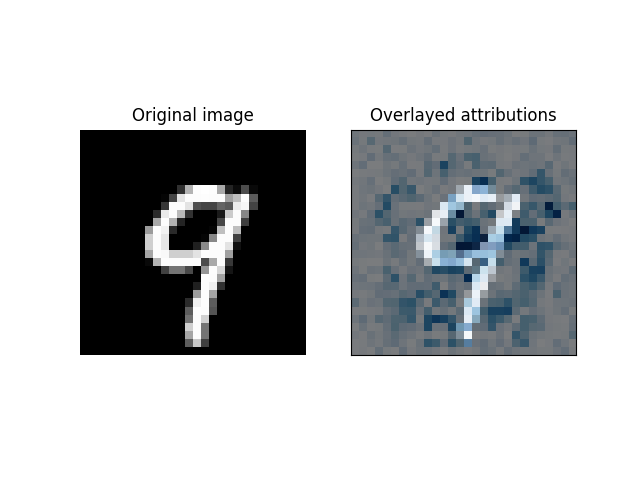
\includegraphics[width=.6\linewidth]{img/saliency_flat/9.png}
    \caption{Digits and saliency maps for digits 0,4, and 9.}\label{fig:flatten-attributions}
\end{figure}

The simplest MLP model that simply flattens the image to a 784-element vector was analyzed using the saliency method.
The resulting saliency maps for example digits are shown on fig~\ref{fig:flatten-attributions}.
From these maps it is possible to deduce the model's ``reasoning'' when classifying certain classes.

For example, with digit 0, it pays great attention to the area in the middle. That is because, contrary to other digits, 0 has a big empty space in the middle.
We suspect that the model has learnt to recognize this empty middle space and associate it with the digit 0, which is in line with human intuition.

Similarly, for digit 4, there is also an open space at the top, to which the model pays great attention. 
The model is at the same time not paying much attention to the bottom area, because with the digit 4, it does not contain many discernable characteristics.

In the example with the digit 9, a lot of model's attention is focused on the crossing present in the digit. At the same time, the model is looking at the bottom, because sometimes the digit 9 is drawn with a ``hook'' there.

With all of the digits, we are satisfied that the model is not paying attention to much of the edge pixels, meaning thet it does not focus on the background too much,
which is the correct behaviour. 

\subsubsection{LBP}
\subsubsection{HOG}

\begin{figure}[ht]\centering
    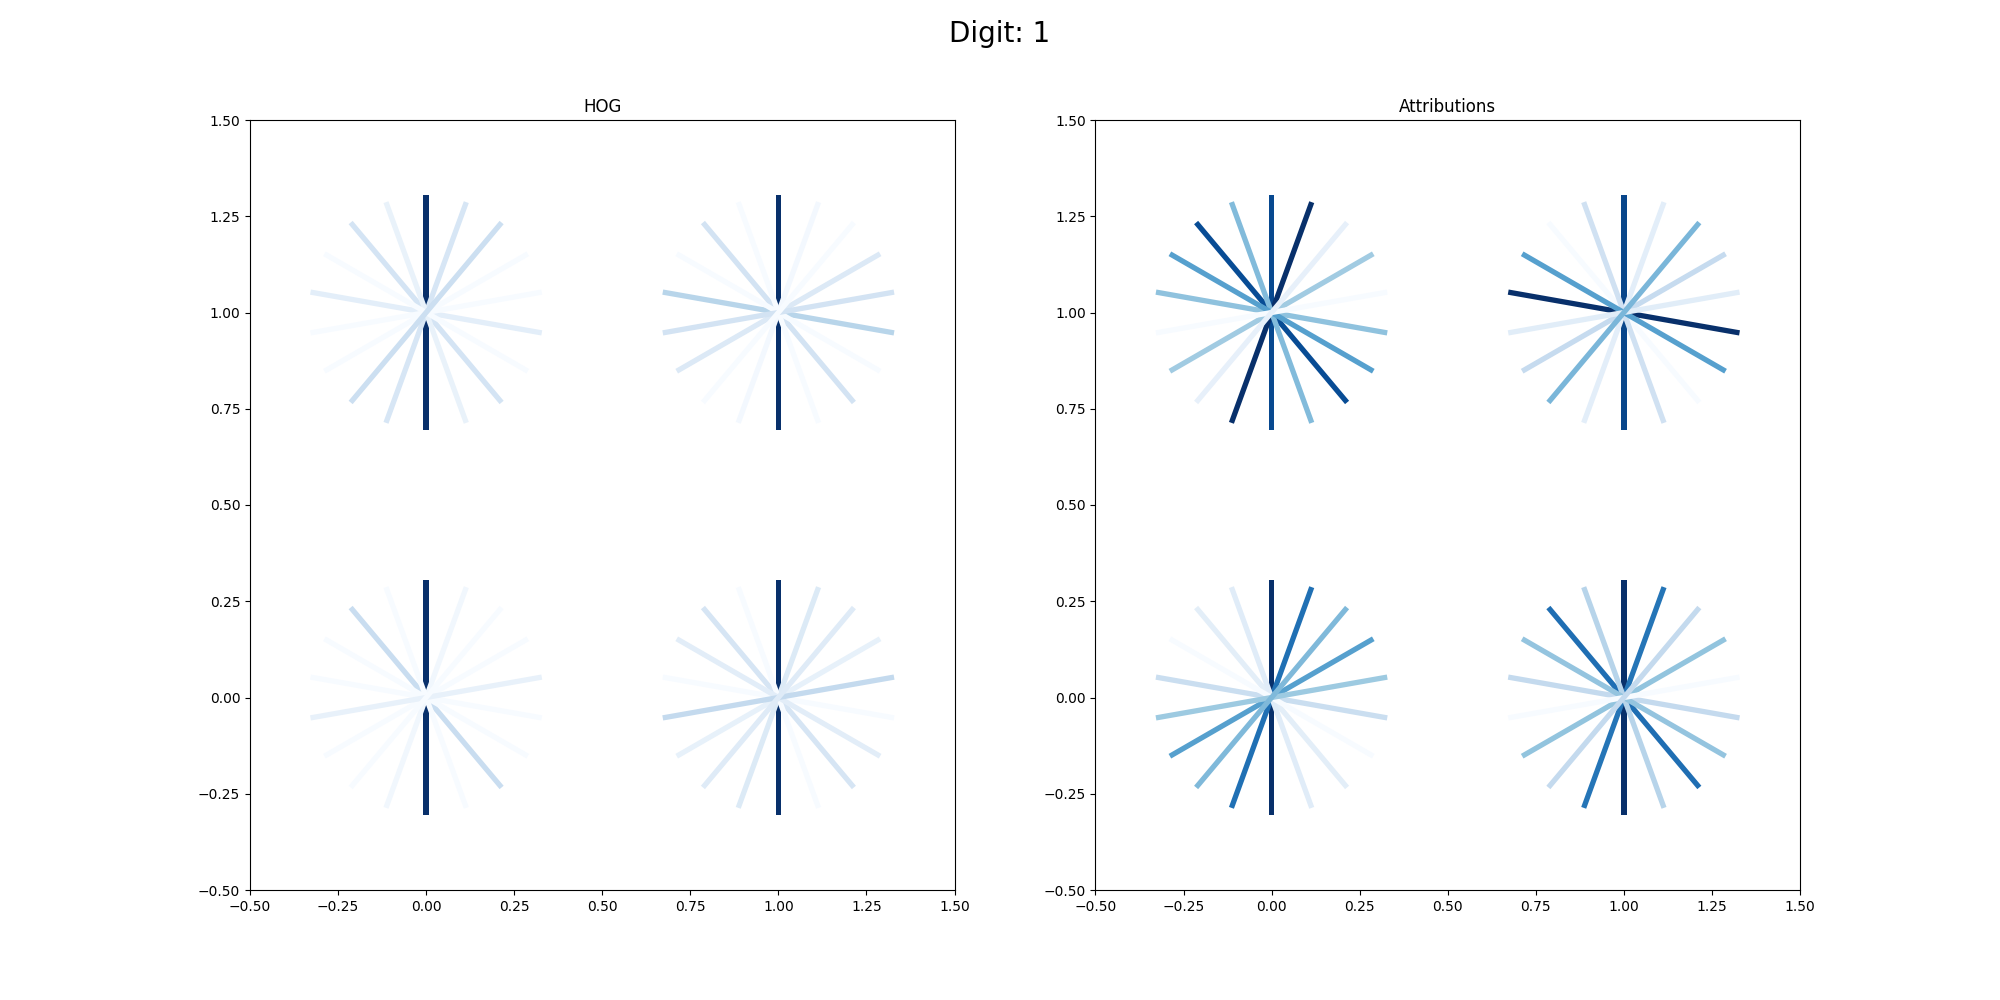
\includegraphics[width=.6\linewidth]{img/saliency_hog/1.png}
    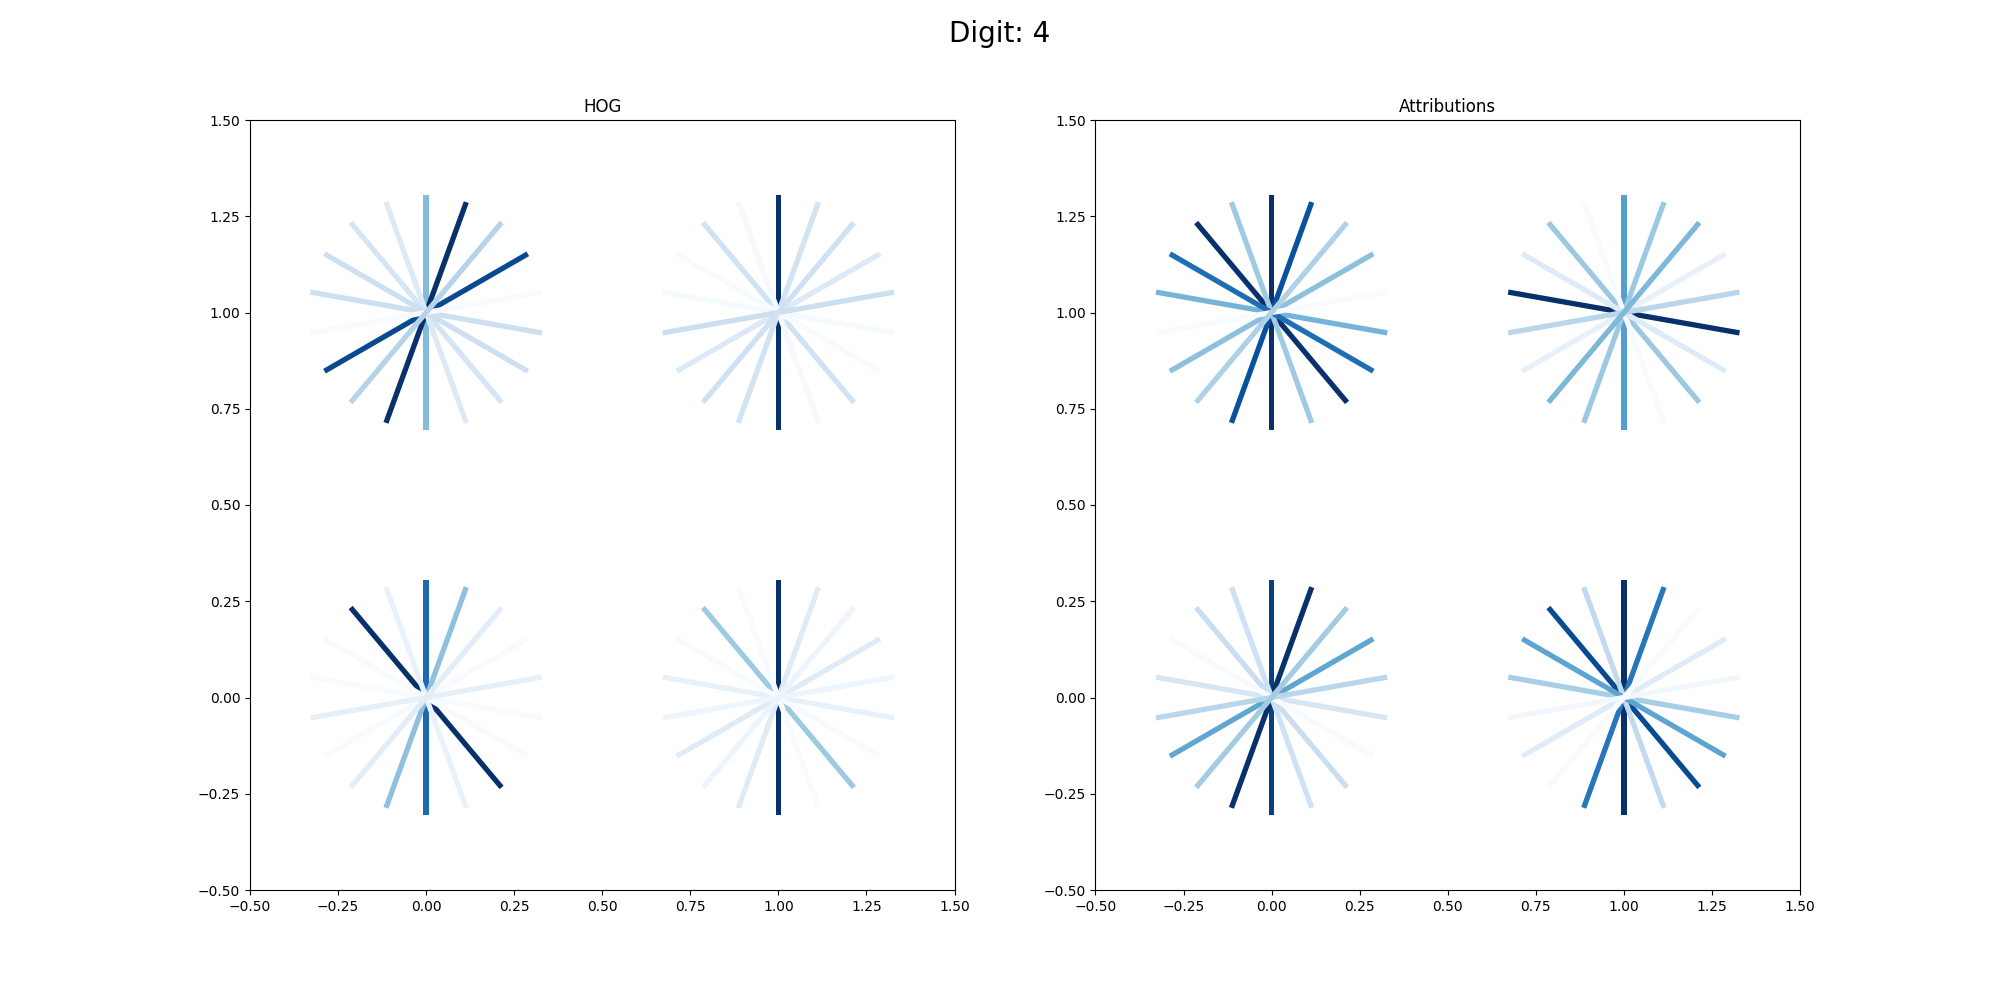
\includegraphics[width=.6\linewidth]{img/saliency_hog/4.png}
    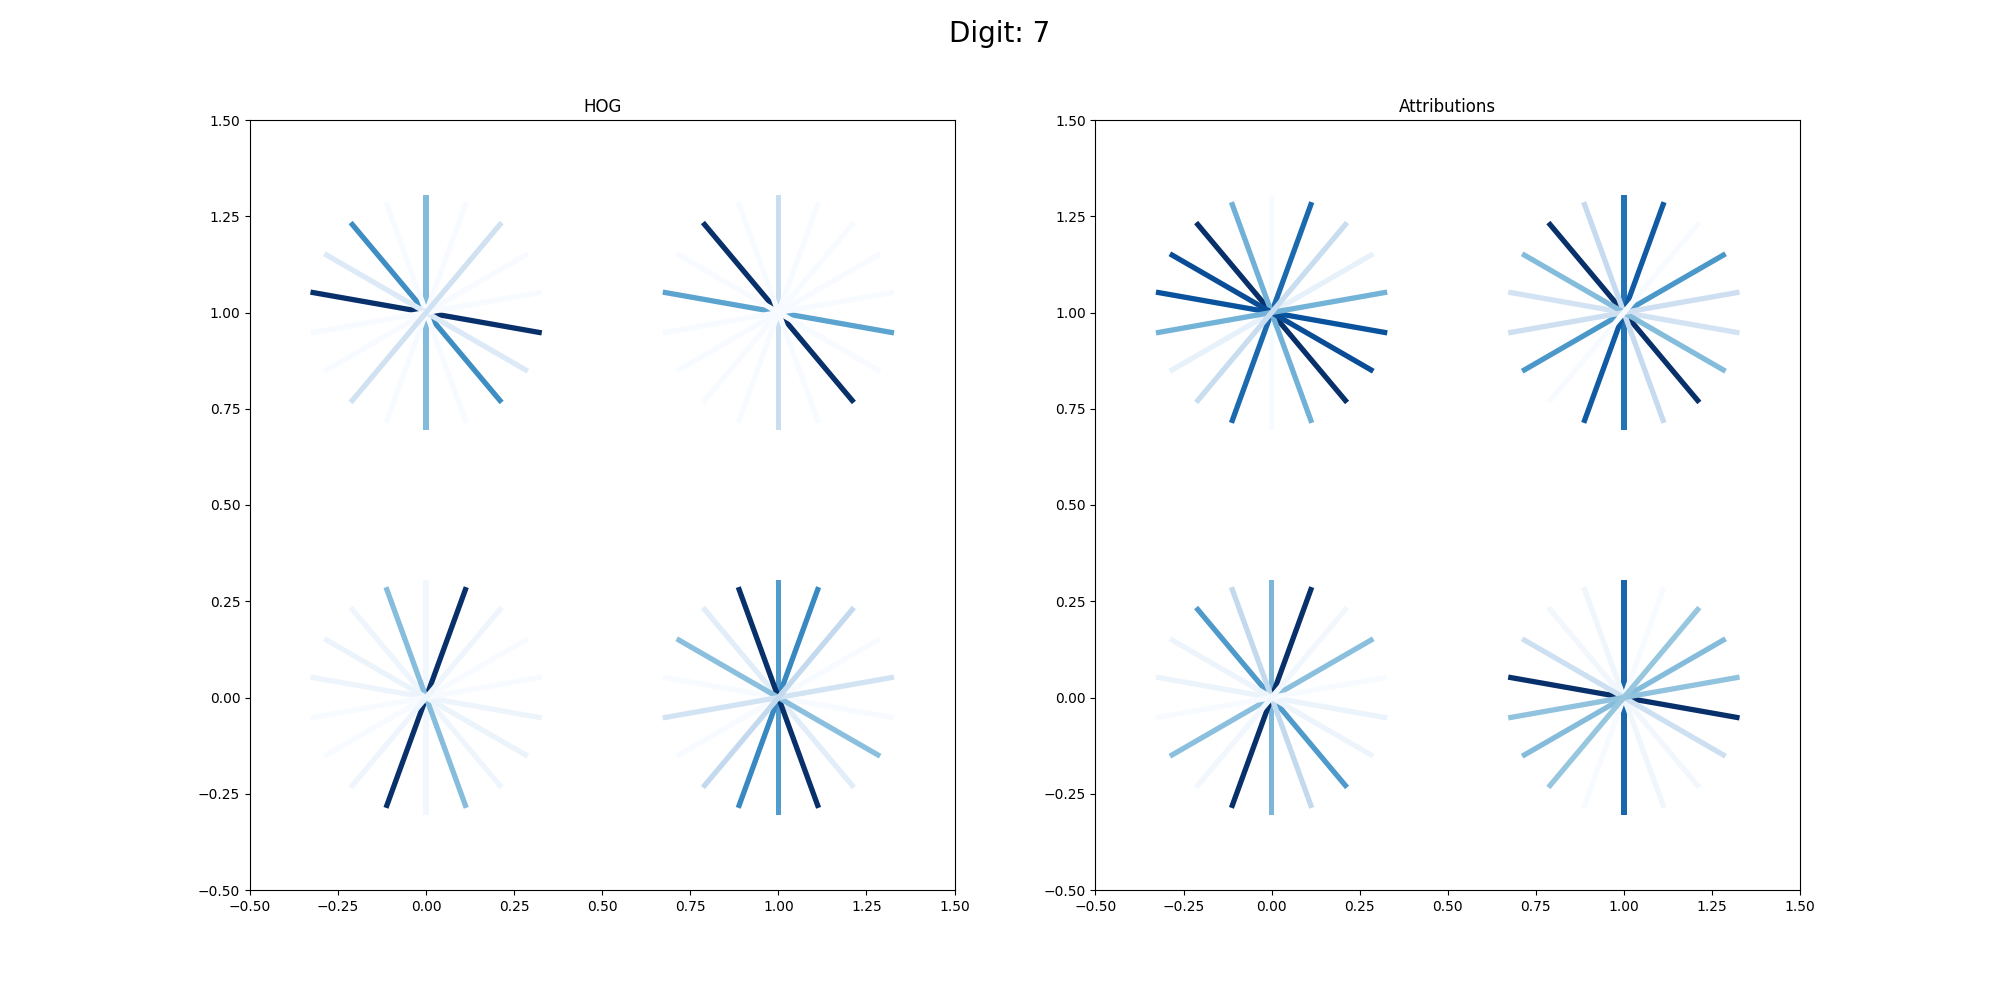
\includegraphics[width=.6\linewidth]{img/saliency_hog/7.png}
    \caption{HOG values and gradient attributions for digits 1,4, and 7.}\label{fig:hog-attributions}
\end{figure}

The MLP that operated on features extracted using the histogram of oriented gradients was analyzed using the saliency method to determine
if the directions that have the influence on the model are actually those present in the digits.
The results are visualized on fig.~\ref{fig:hog-attributions}.

As expected, the features present in the digits are in fact those that have an impact on the model's answer.
However, the model also pays attention to some other directions, which are not present in the input digit.
We assume this behavior to be caused by model determining these features to be most differentiating between similar digits.
Because of this, such features have a big impact in the models decision.

\subsection{MNIST CNN classifier}\label{subsec:experiment-mnist-cnn}

\begin{figure}[ht]\centering
    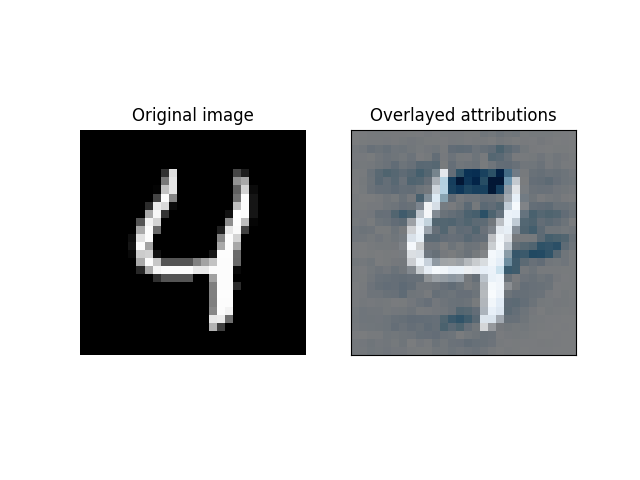
\includegraphics[width=.6\linewidth]{img/saliency_mnist/4.png}
    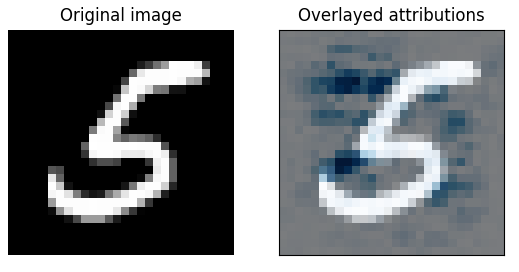
\includegraphics[width=.6\linewidth]{img/saliency_mnist/5.png}
    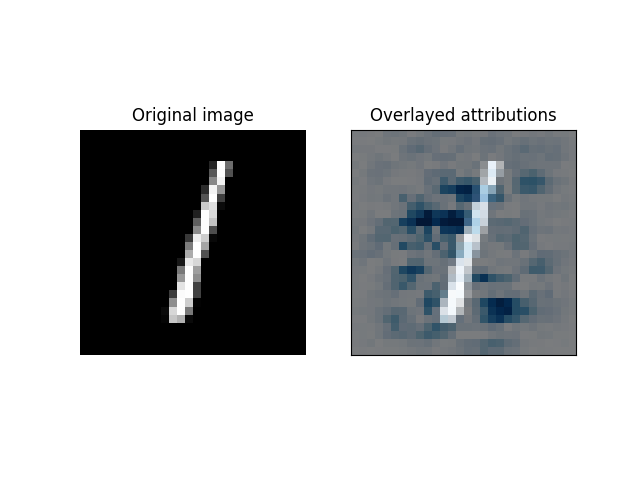
\includegraphics[width=.6\linewidth]{img/saliency_mnist/1.png}
    \caption{Saliency maps of chosen MNIST digits}\label{fig:mnist-cnn-saliency}
\end{figure}

The CNN for recognizing handwritten digits from the MNIST dataset was analyzed using the saliency methods.
The resulting saliency maps are visualized on fig.~\ref{fig:mnist-cnn-saliency}.
The blue pixels show the areas that most influence the model's predictions.

Unexpectedly, the obtained saliency maps predominantly highlight background pixels adjacent to the digits
rather than the digits themselves.
One plausible explanation of this phenomenon is that the CNN has learned the absence of pixels in a specific region as
important information for its classification decisions --- for example, the digits 4 and 5 are characterized by the lack of the closed regions.
If one was to add pixels to these areas 4 would turn into a 9, and 5 would turn into a 6.
Therefore, these areas are highlighted as important to the classification results, because it is essential that no pixels exist in those areas.
Such behaviour might suggest that the model is not recognizing the digits by their shape directly, but rather by elimination --- i.e.\ an important characteristic of a digit 4 is that it is not a 9.

The background pixels might also provide contextual information about the area around the digit.
This is especially important in shape recognition tasks, such as digit recognition.
For example, the top bar at the digit 5 is oriented to the right-hand side, however, there are pixels highlighted to the left-hand side.
That is because for a line to be considered as oriented to the right, there need to be both a presence of pixels to the right, and a lack of them to the left.
Therefore, the background also needs to be considered in order to correctly determine the shape characteristics and boundaries.

Another unfortunate possibility of such behaviour may be some issues with the model.
Overfitting could cause the model to focus on some background pixels, that are not really representative of the digit features.
However, it should be noted that during the model evaluation, we did not observe a drop in accuracy on the test set during training --- a typical sign of overfitting.
Additionally, the performance of the model on the testing data was satisfactory, which speaks against the potential issues with the model.

To further investigate this model we used Integrated Gradients method as well.
\begin{figure}[h]\centering
    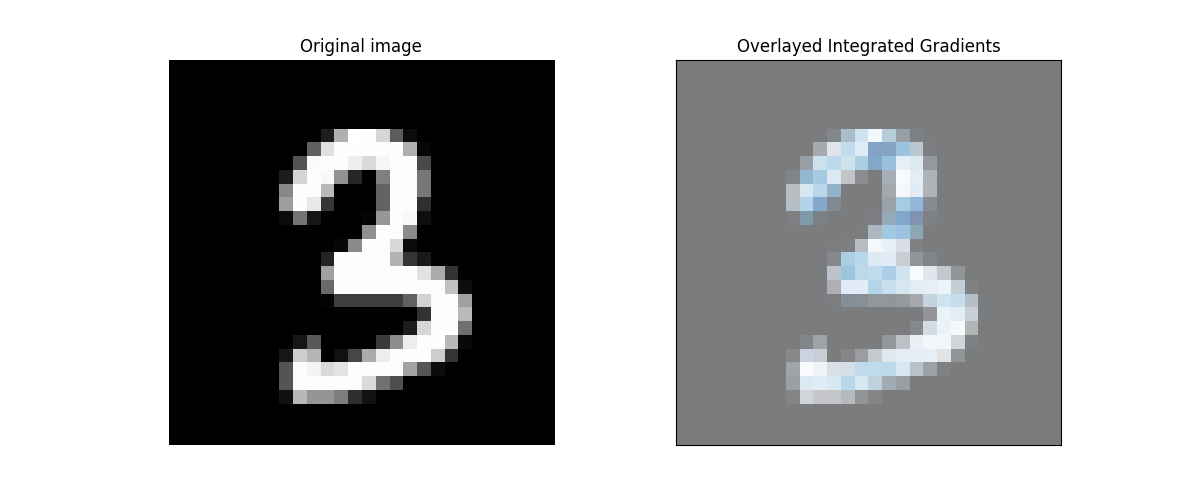
\includegraphics[width=.6\linewidth]{img/integrated_grad/mnist_CNN/3}
    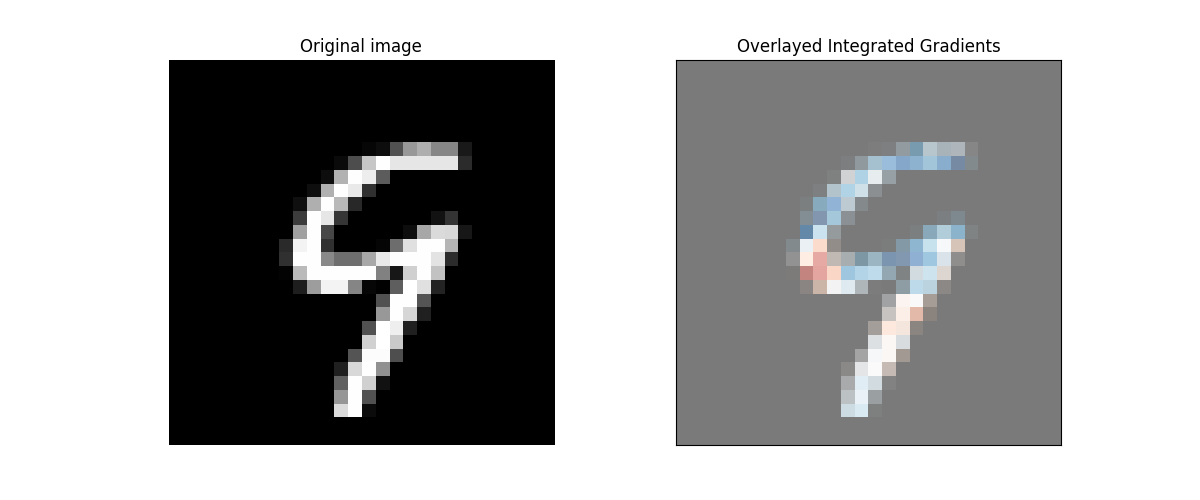
\includegraphics[width=.6\linewidth]{img/integrated_grad/mnist_CNN/4_again2}
    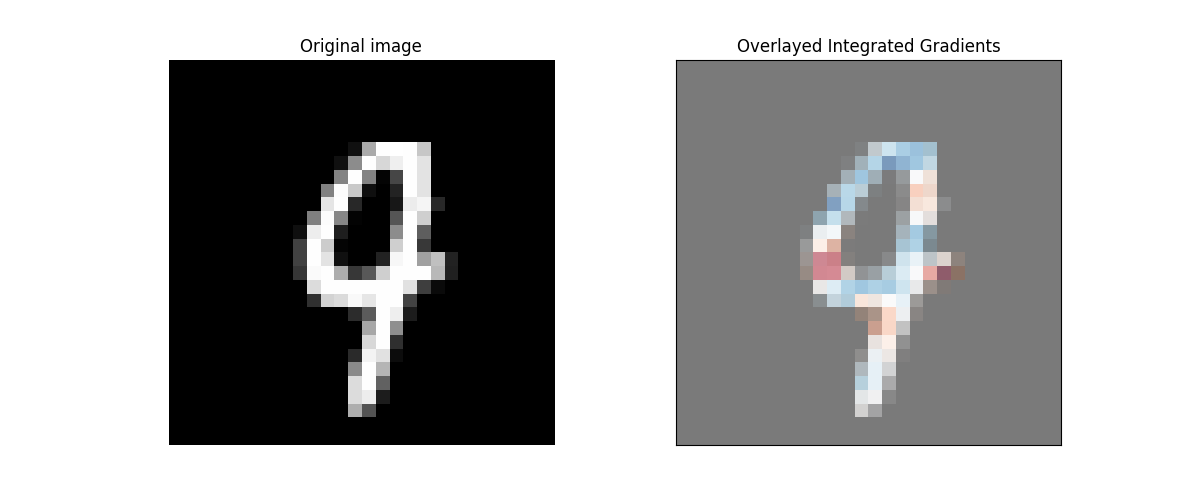
\includegraphics[width=.6\linewidth]{img/integrated_grad/mnist_CNN/9}
    \caption{Integrated Gradients of chosen MNIST digits}\label{fig:mnist-cnn-integrated-grad}
\end{figure}
Similar to the previous example, the blue pixels indicate the areas that most influence the model's predictions and red pixels the least.

Integrated Gradients provide a clear depiction and explanation of the areas considered by the model during prediction.
Examples on fig.~\ref{fig:mnist-cnn-integrated-grad} illustrate that digit 3 is most recognizable by its distinctive curves, aligning with human perception of this numeral's defining features.
Additionally, integrated gradients reveal subtle distinctions between visually similar digits.
For instance, in digits 4 and 9, although they share similarities, the connected top part plays a crucial role in differentiation.
Moreover, this method highlight areas in the digits where the model might make errors or find ambiguity.
In the central regions of digits 4 and 9, represented by less intense colors (notably red), the model's certainty decreases.
This suggests that these regions resemble characteristics of multiple digits, potentially leading to misclassification.

To further enhance our analysis, we employed the SLIC superpixel method.

\begin{figure}[h]\centering
    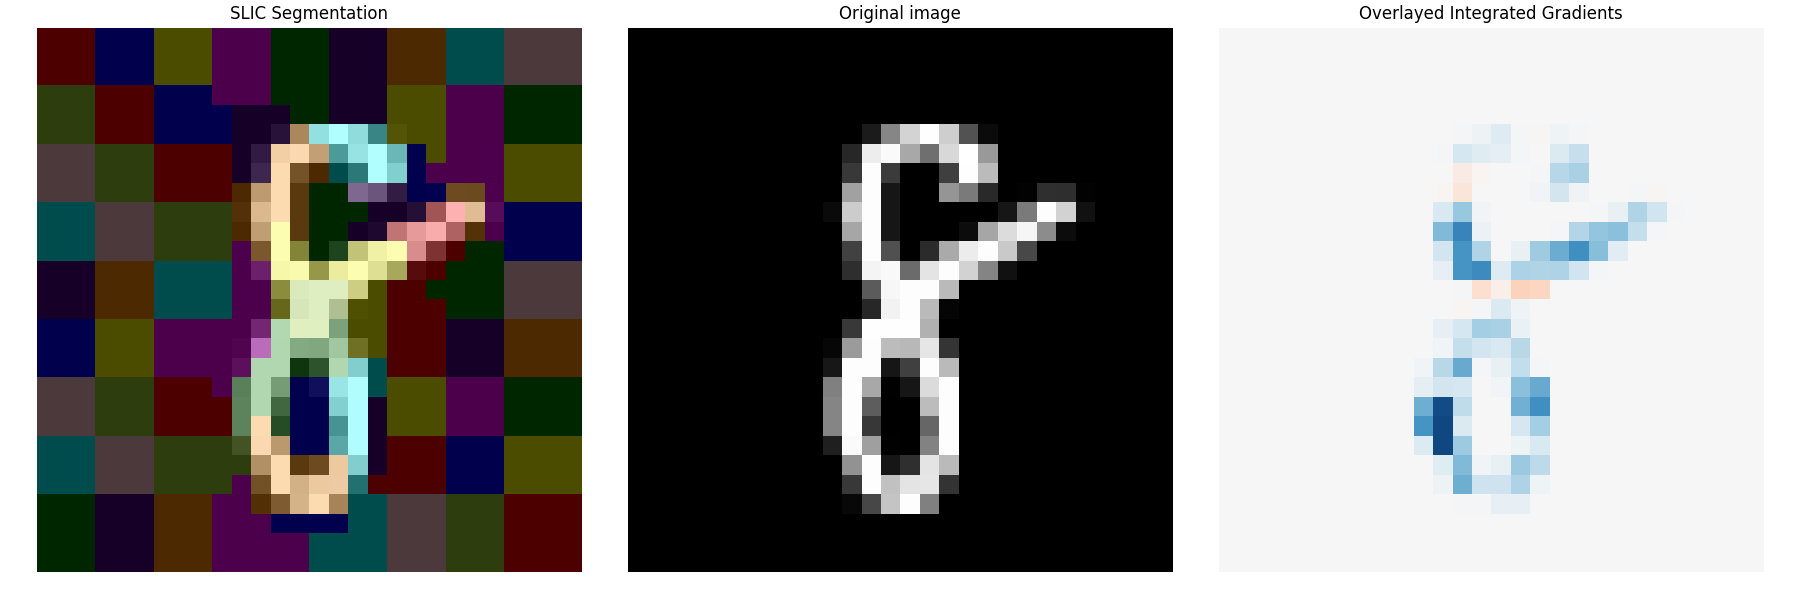
\includegraphics[width=.6\linewidth]{img/SLIC/mnist/8}
    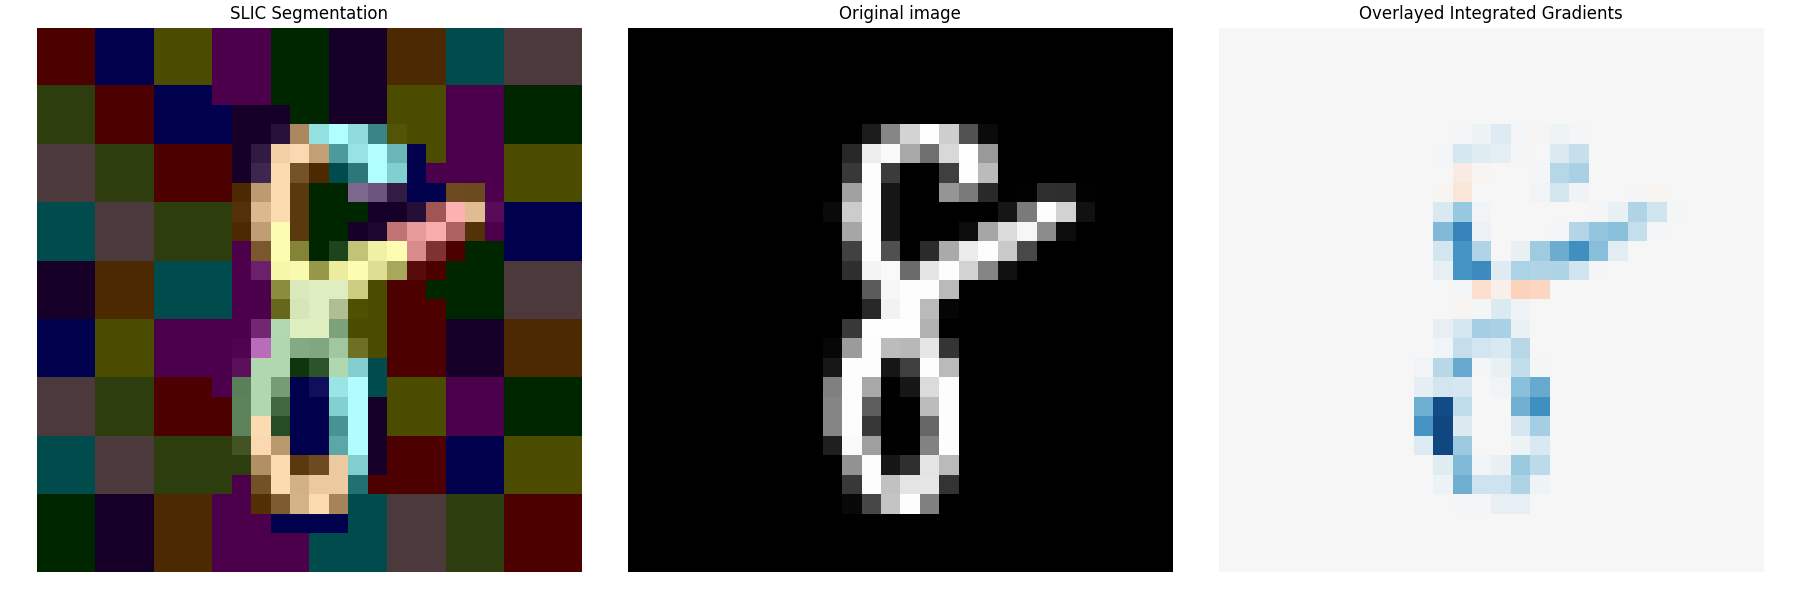
\includegraphics[width=.6\linewidth]{img/SLIC/mnist/8_1}
    \caption{SLIC method on chosen MNIST digits}\label{fig:mnist-cnn-slic}
\end{figure}

SLIC generates segmented regions that highlight the spatial importance of different parts of the digit.
By focusing on these superpixels, we gain insights into which regions the model prioritizes when making decisions.
For example on the fig.~\ref{fig:mnist-cnn-slic} we observe that in case of classification fo difit 8, the most crucial part is the center, where two curves cross each other.
Integrating this method enhances model transparency and improves understanding of the model prediction.

Finally, we applied perturbation technique to various digits to assess how the model would classify them if parts of the images were covered.

\begin{figure}[ht]\centering
    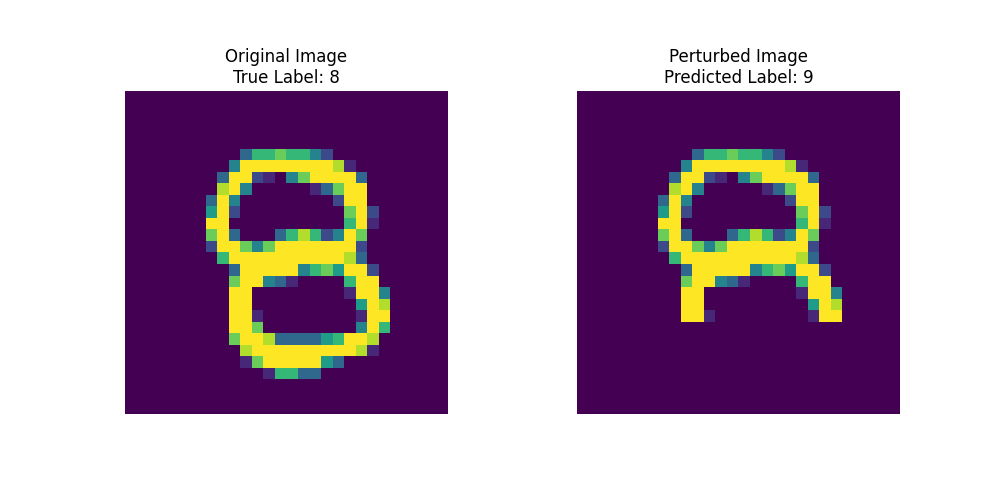
\includegraphics[width=.6\linewidth]{img/counterfacts/MNIST/cover_bottom/img_1}
    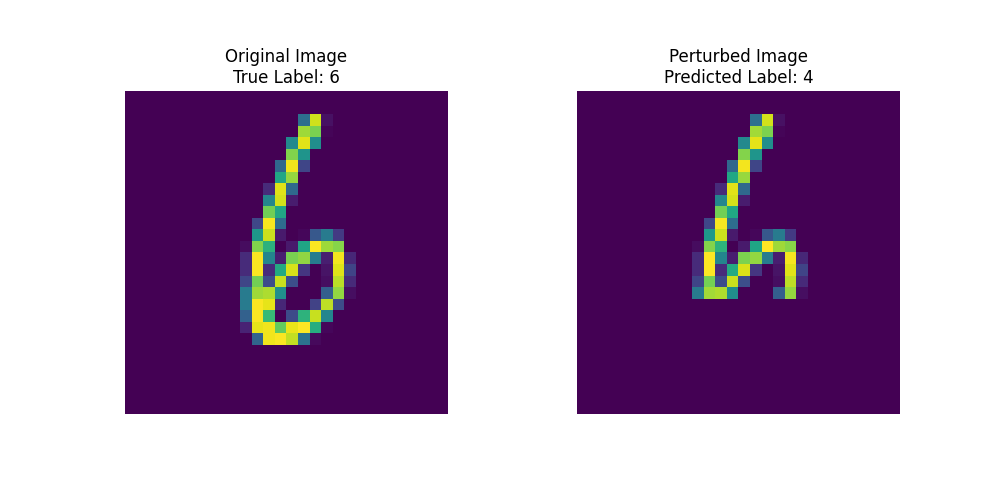
\includegraphics[width=.6\linewidth]{img/counterfacts/MNIST/cover_bottom/img_3}
    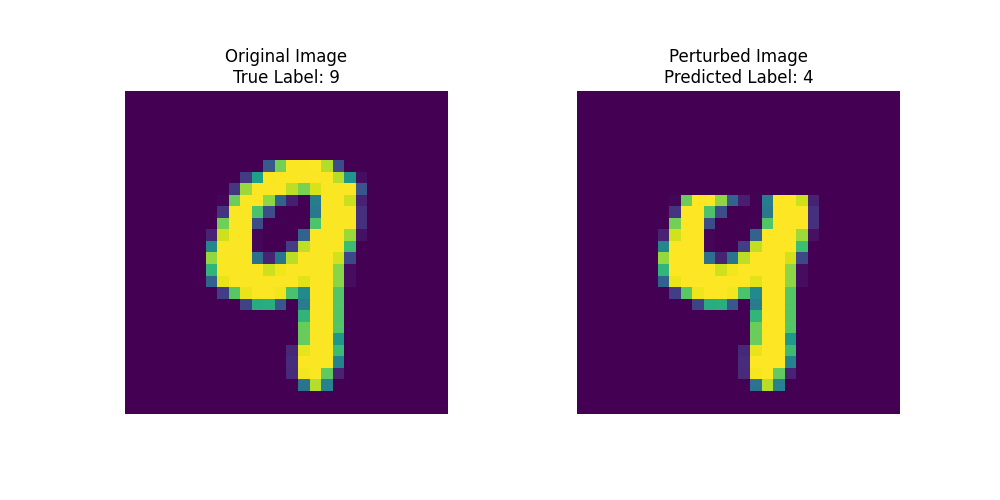
\includegraphics[width=.6\linewidth]{img/counterfacts/MNIST/cover_top/img_10}
    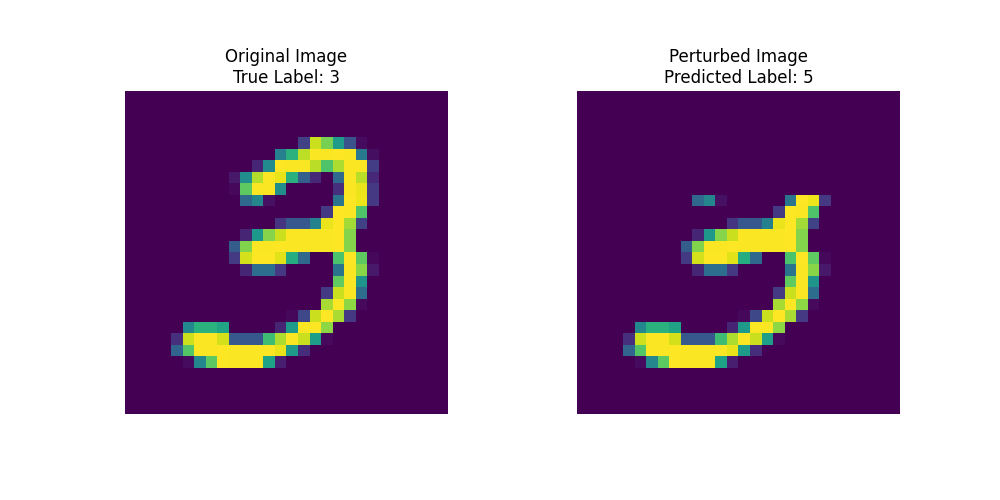
\includegraphics[width=.6\linewidth]{img/counterfacts/MNIST/cover_top/img_3}
    \caption{Perturbation method on chosen MNIST digits}\label{fig:mnist-cnn-counterfacts}
\end{figure}

We can observe on the fig.~\ref{fig:mnist-cnn-counterfacts} that covering the bottom part of the digit 8 leads the model to classify it as 9.
Similarly, covering part of the digit 6 results in a misclassification as 4.
These observations highlight specific regions of the image that significantly influence the model's predictions.
The perfect example of explanation of the figures on~\ref{fig:mnist-cnn-integrated-grad} is with the coverage of the top part of 9, which results in misclassification as 4.
Therefore, it proves the fact that the top part of digit 9 is most influential.
Similarly, in another instance, the absence of the top curve in a digit causes the model to predict 5 instead of 3.

This technique is a powerful tool for error analysis and diagnosis.
Using it demonstrates how small changes in input can affect model predictions and trustworthiness.

\subsection{CIFAR10 CNN classifier}\label{subsec:experiment-cifar}

\begin{figure}[ht]\centering
    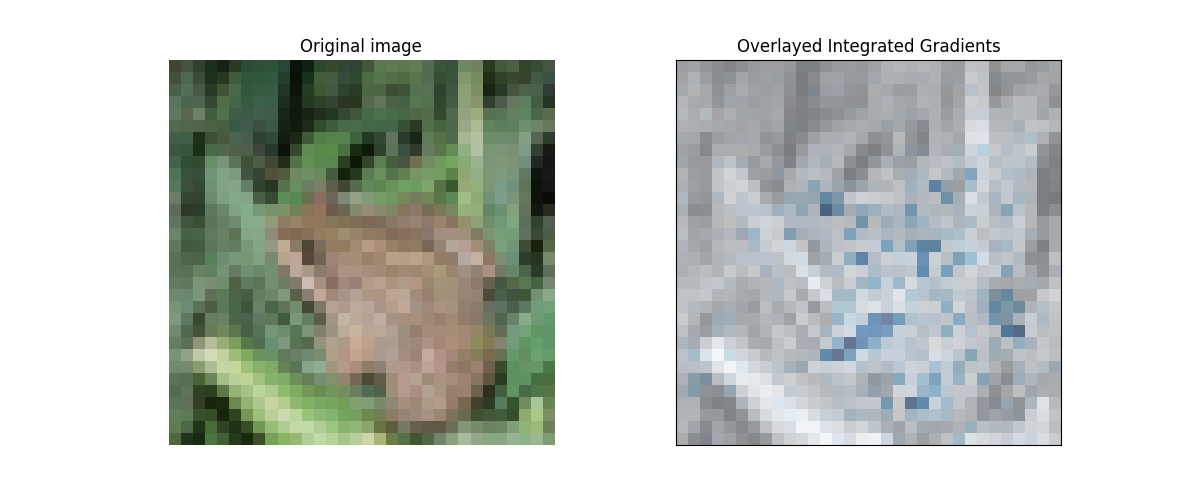
\includegraphics[width=.6\linewidth]{img/integrated_grad/cifar_CNN/frog}
    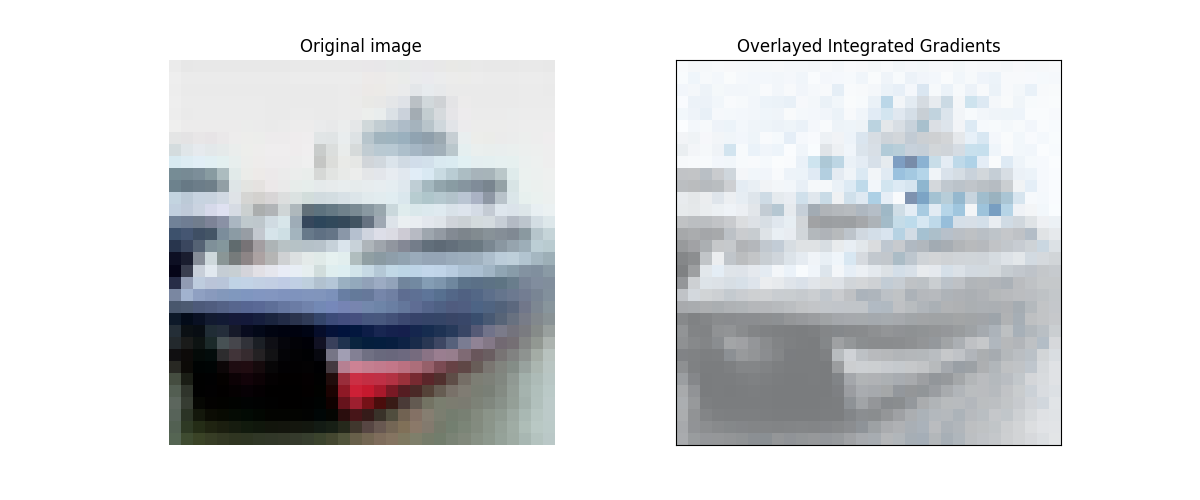
\includegraphics[width=.6\linewidth]{img/integrated_grad/cifar_CNN/ship}
    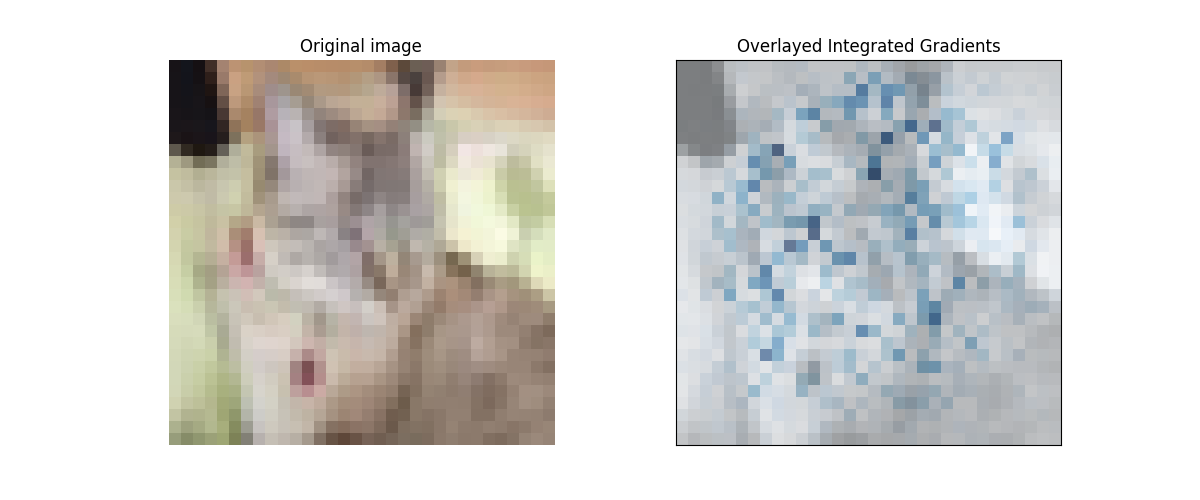
\includegraphics[width=.6\linewidth]{img/integrated_grad/cifar_CNN/cat2}
    \caption{Integrated Gradients of chosen CIFAR images}\label{fig:cifar-cnn-int-grad}
\end{figure}
In our exploration of CNN model trained on the CIFAR10 dataset, we utilized Integrated Gradients to enhance our understanding of how these models classify objects within images.

Integrated Gradients highlight significant object features within CIFAR10 images, offering valuable insights into the model's decision-making process.
This focus is particularly effective for images where objects are distinct and prominently displayed, such as the frog and cat examples on fig.~\ref{fig:cifar-cnn-int-grad}.
Here, the model accurately identifies and highlights features of these objects, enhancing interpretability.
However, challenges arise with images like the ship, where the object’s distinction from the background is less pronounced.
In such cases, Integrated Gradients struggle to clearly delineate object boundaries due to color similarity or background complexity.

Addressing this challenge with background interference may involve enhancing model robustness through data augmentation or adapting interpretability techniques tailored to complex visual environments.
Such insights are crucial for deploying CNN models in real-world scenarios, such as autonomous systems, medical diagnostics, and security surveillance, where accurate object recognition amidst varying environmental conditions is paramount.

To further investigate model prediction, we implemented the SLIC super-pixel method.

\begin{figure}[ht]\centering
    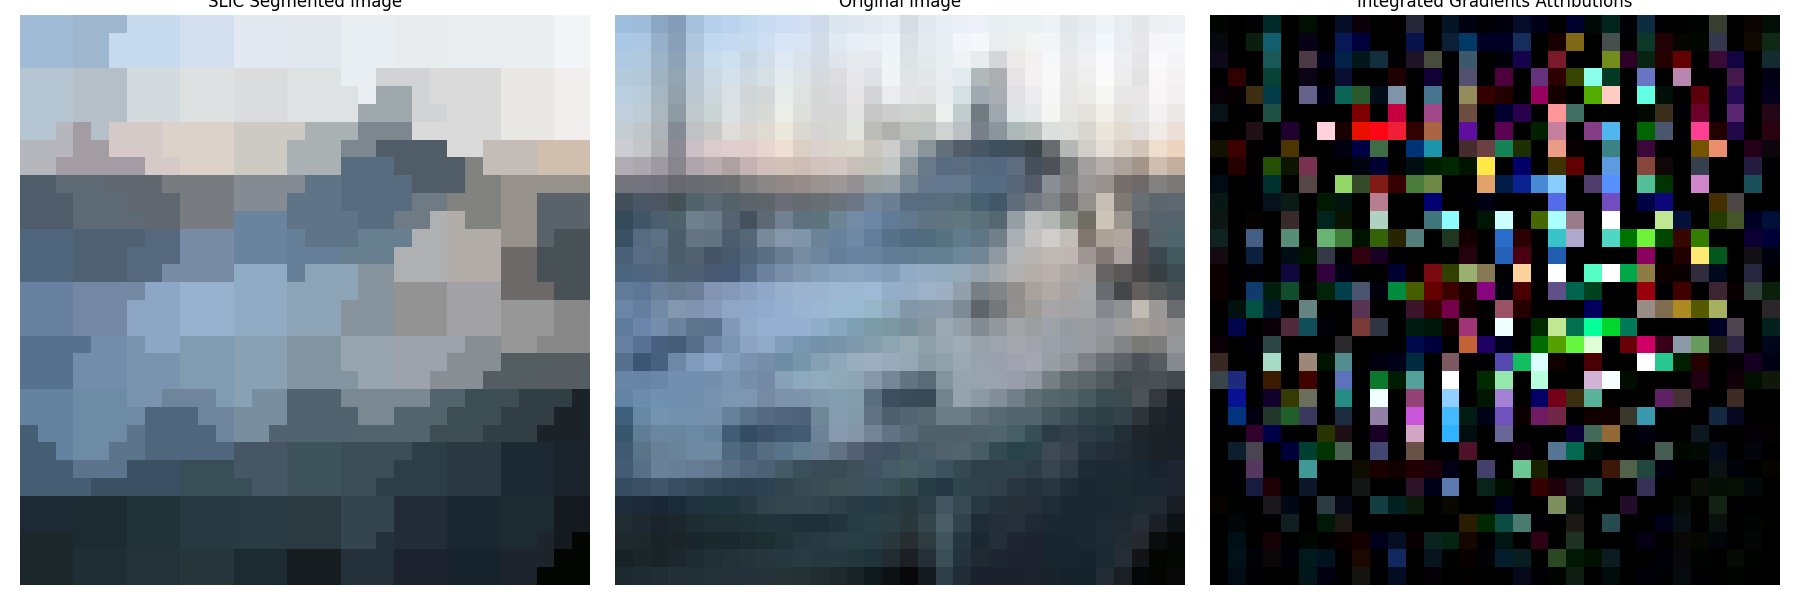
\includegraphics[width=.6\linewidth]{img/SLIC/cifar/img_2}
    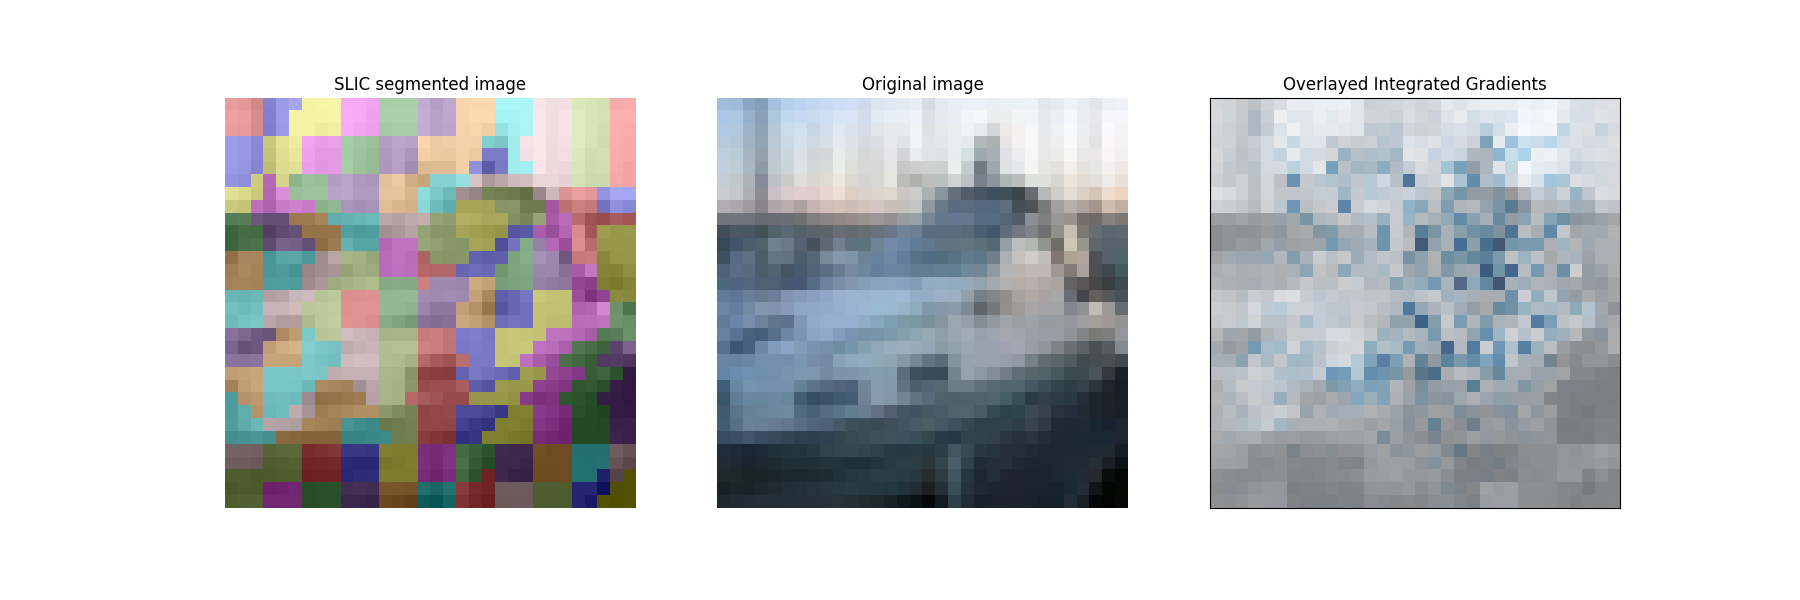
\includegraphics[width=.6\linewidth]{img/SLIC/cifar/img_3}
    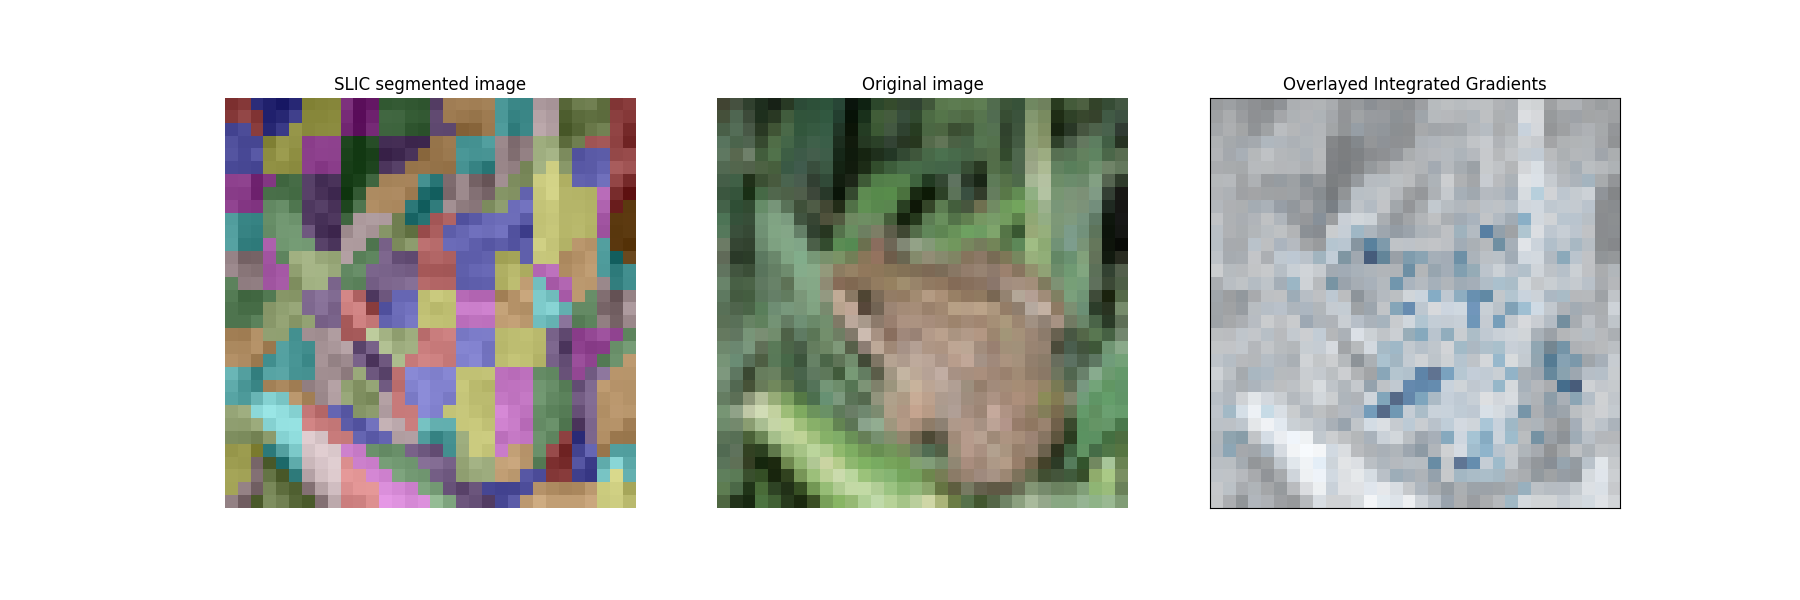
\includegraphics[width=.6\linewidth]{img/SLIC/cifar/img_5}
    \caption{SLIC method on chosen CIFAR images}\label{fig:cifar-cnn-slic}
\end{figure}

SLIC by generating segmented regions, allows us to gain insights into which areas of the image influence a model the most.
In this case, comparing the examples with implemented SLIC method on~\ref{fig:cifar-cnn-slic} to the examples on ~\ref{fig:cifar-cnn-int-grad}, we can notice more pixels that were highlighted and the image to be more separated into regions.
However, the results aren't that much more visible like in the example for the MNIST dataset, yet they add a little more insight into understanding model's prediction.

To further assess the robustness and reliability of our CNN model trained on the CIFAR10 dataset, we implemented perturbation techniques.
Specifically, we investigated how the model's classification performance changes when images are slightly rotated.
This analysis helps us understand the model's sensitivity to variations in input and its reliance on specific visual features for accurate predictions.

\begin{figure}[ht]\centering
    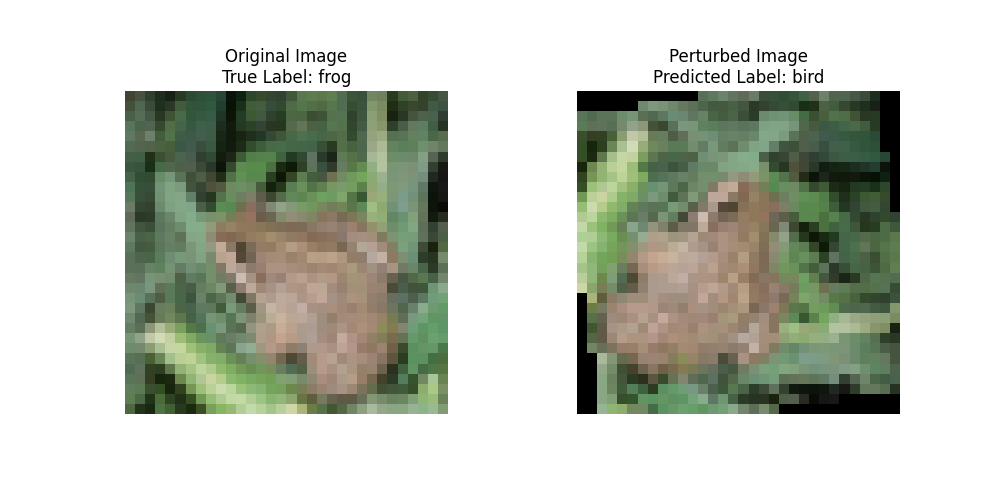
\includegraphics[width=.6\linewidth]{img/counterfacts/CIFAR/img_2}
    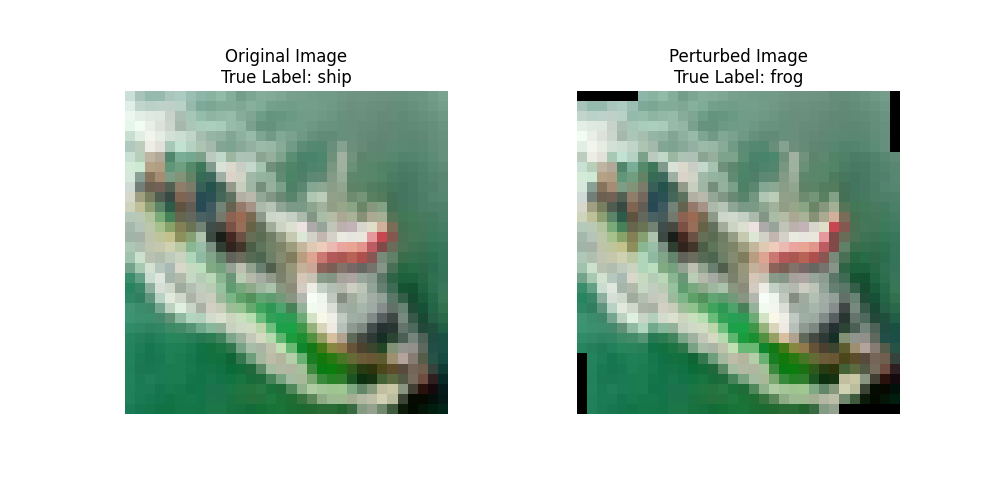
\includegraphics[width=.6\linewidth]{img/counterfacts/CIFAR/img_7}
    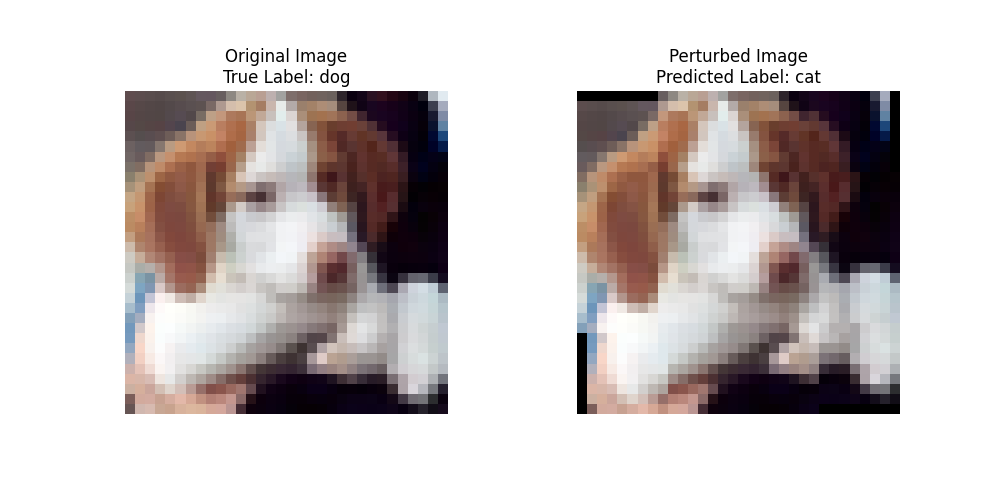
\includegraphics[width=.6\linewidth]{img/counterfacts/CIFAR/img_8}
    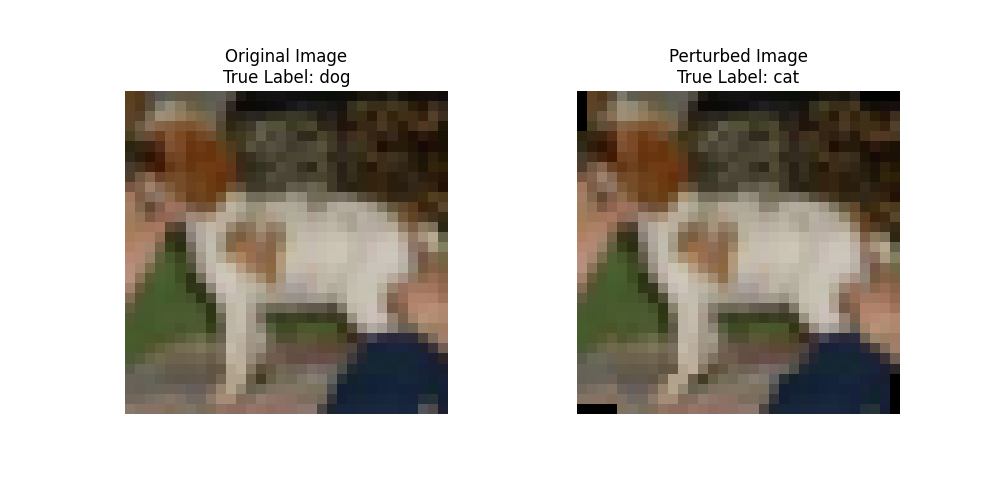
\includegraphics[width=.6\linewidth]{img/counterfacts/CIFAR/img_6}
    \caption{Perturbation on chosen CIFAR images}\label{fig:cifar-cnn-peturbation}
\end{figure}

The perturbation results, depicted on fig.~\ref{fig:cifar-cnn-peturbation}, provide a detailed view of the model's behavior under rotational transformations.
For images where the object of interest is prominently displayed and distinct from the background, the model demonstrates robustness to significant rotations.
For instance, the frog image requires a rotation above 82.15 degrees before the model misclassifies it.
This indicates that the model reliably recognizes the frog based on its salient features despite substantial perturbations.

However, images with less distinct objects or complex backgrounds show vulnerability to even minor rotations.
The ship image, for instance, is misclassified as a frog with only a 3.65-degree rotation.
This misclassification likely arises due to the green background, which the model mistakenly associates with the frog class.
This scenario highlights the model's susceptibility to background interference when object and background colors are similar.
The model also shows difficulty distinguishing between visually similar classes under slight perturbations.
As seen on fig.~\ref{fig:cifar-cnn-peturbation}, small rotations (2.47 and 3.85 degrees) cause the model to misclassify a dog as a cat.
This suggests that the model's feature extraction process may not effectively differentiate between subtle visual differences in closely related classes.
Moreover, in this experiment the model was working on the not augmented data, due to this the recognition of these images might not be as expected.

These findings underscore the importance of rigorous model evaluation under diverse conditions to ensure reliability in practical applications.
Models deployed in different fields such as surveillance or medical imaging must maintain high accuracy despite variations in input, making perturbation analysis a critical component of model validation.

Addressing this challenge through targeted training enhancements and interpretability techniques can lead to more robust and reliable models suited for complex real-world tasks.

\section{Summary}\label{sec:summary}
Summarize the main conclusions and suggest future work.

\section{References}\label{sec:references}

\bibliographystyle{IEEEtran}
\bibliography{references}

\end{document}
